\pdfoutput=1
%%%%%%%%%%%%%%%%%%%%%%%%%%%%%%%%%%%%%% 
% Multiplicative domain poster
% Created by Nathaniel Johnston
% August 2009
% http://www.nathanieljohnston.com/index.php/2009/08/latex-poster-template/
%%%%%%%%%%%%%%%%%%%%%%%%%%%%%%%%%%%%%%
% This very blank poster was created by Katherine M. Kinnaird from Nathaniel Johnston's poster template and style file(see above). The style file was edited by Sarah E. Wright.
% It makes use of a variety of formatting tools, but is by no means complete.
% You will need to use the style file in this folder.
% The Dartmouth Grad Studies and the Math Department logos are in this folder
% March 2013
%%%%%%%%%%%%%%%%%%%%%%%%%%%%%%%%%%%%%%

\documentclass[
                20pt,
                final,
                hyperref={%
                    breaklinks=true,%
                    letterpaper=true,%
                    colorlinks,%
                    bookmarks=false%
                }]{beamer}

% Recommended, but optional, packages for figures and better typesetting:
\usepackage{microtype}
\usepackage{graphicx}
\usepackage{booktabs} % for professional tables

% For theorems and such
\usepackage{mathtools}

\usepackage{nicefrac}

\makeatletter
\@namedef{ver@everyshi.sty}{}
\makeatother

\usepackage{tikz}
\usepackage{pgfplots}
\pgfplotsset{compat=newest}
\DeclareUnicodeCharacter{2212}{−}
\usepgfplotslibrary{groupplots,dateplot}
\usetikzlibrary{patterns,shapes.arrows}
\usetikzlibrary{backgrounds}
\usetikzlibrary{arrows}
\usetikzlibrary{shapes,shapes.geometric,shapes.misc}

\usepackage{calc}
\usepackage{lmodern}
\usepackage{exscale}

%\usepackage[centering,text={15.5cm,24cm}]{geometry}
\usepackage{graphicx}
\usepackage[all]{xy}
%\usepackage{mathrsfs}
\usepackage{marvosym}
%\usepackage{stmaryrd}
\usepackage[scr]{rsfso}
\usepackage{srcltx}

\usepackage[shadow,textwidth=1.8cm]{todonotes}

\usepackage{changepage}
\usepackage{pstricks}

\usepackage{amsfonts,amsmath,amssymb,amscd,amsthm}
%\usepackage{amsaddr}
\usepackage{enumerate}
\usepackage[all]{xy}
\usepackage{mathtools}

\usepackage{xparse}
\usepackage{float}

%\usepackage[
%    %fontsize=30.2pt
%    ]{fontsize}
%\newcommand{\fontstorlek}{60pt}
%\changefontsize[\fontstorlek]{\fontstorlek}

\usepackage{physics}
\usepackage{dsfont}
\usepackage{bbm}
\usepackage{bm}
\usepackage{tabu}
\usepackage{booktabs}
\usepackage{tensor}
\usepackage{textcomp}
\usepackage{subcaption}
\usepackage[group-separator={,}]{siunitx}

\usepackage{lipsum}

%\usepackage[T1]{fontenc}
\usepackage{inputenc}
\usepackage{multicol}
\usepackage{ifthen}
%\usepackage{tikz,tikz-cd}
%\usetikzlibrary{arrows,backgrounds,calc,decorations.pathreplacing}



% The ICML2022 package uses the natbib package
%\usepackage[]{natbib}
%\setcitestyle{numbers, open={[[}, close={]]}}

%\usepackage{better_poster}
\usepackage{tikz}
\usetikzlibrary{calc}

\usepackage{graphicx}
\usepackage{enumerate}
\usepackage[all]{xy}
\usepackage{mathtools}

\usepackage{xparse}
%\usepackage{comment}
\usepackage{float}

\usepackage{physics}
\usepackage{bbm}
\usepackage{tabu}
\usepackage{rotating}
\usepackage{subcaption}

%\usepackage[dvipsnames]{xcolor}

\usepackage{float}

%\usepackage[
%backend=biber,
%style=authoryear-icomp,
%sortlocale=de_DE,
%url=false,
%doi=false,
%eprint=true,
%]{biblatex}
%\addbibresource{./GCNNs.bib}

\usepackage{pgfplots}
\usetikzlibrary{plotmarks,arrows.meta,patterns,shapes.arrows}
\usepgfplotslibrary{patchplots,groupplots,dateplot}
\pgfplotsset{
    % define the layers you need.
    % (Don't forget to add `main' somewhere in that list!!)
    layers/my layer set/.define layer set={
        background,
        main,
        foreground
    }{
        % you could state styles here which should be moved to
        % corresponding layers, but that is not necessary here.
        % That is why wo don't state anything here
    },
    % activate the newly created layer set
    set layers=my layer set,
    compat=newest,
}
\usepackage{grffile}
\usepackage{amsmath}

%\usepackage{icml2022}

\usepackage{natbib}
%\usepackage{biblatex}


%\usepackage[
%            %pagebackref=true,
%            breaklinks=true,
%            letterpaper=true,
%            colorlinks,
%            bookmarks=false
%            ]{hyperref}

% if you use cleveref..
\usepackage[capitalize,noabbrev]{cleveref}
%%% Local Variables:
%%% mode: latex
%%% TeX-master: "mnist_paper"
%%% End:


\DeclareCaptionFormat{custom}
{%
    %\textbf{#1#2}\textit{\small #3}
    \rmfamily{\small{\color{dblue}#1#2\color{black} #3}}
}
\captionsetup{format=custom}

\newtheorem*{namedtheorem}{\theoremname}
\newcommand{\theoremname}{testing}
\newenvironment{named}[1]{\renewcommand\theoremname{#1}
    \begin{namedtheorem}}
    {\end{namedtheorem}}

%\newtheorem{theorem}{Theorem}[section]
%\newtheorem{lemma}[theorem]{Lemma}
%\newtheorem{proposition}[theorem]{Proposition}
%\newtheorem{corollary}[theorem]{Corollary}
%\newtheorem{conjecture}[theorem]{Conjecture}
%\newtheorem{claim}[theorem]{Claim}
%
%\theoremstyle{definition}
%\newtheorem{definition}[theorem]{Definition}
%\newtheorem{construction}[theorem]{Construction}
%\newtheorem{discussion}[theorem]{Discussion}
%\newtheorem{assumption}[theorem]{Assumption}
%\newtheorem{assumptions}[theorem]{Assumptions}
%\newtheorem{convention}[theorem]{Convention}
%\newtheorem{example}[theorem]{Example}
%\newtheorem{examples}[theorem]{Examples}
%\newtheorem*{acknowledgement}{Acknowledgement}

%\theoremstyle{remark}
%\newtheorem{remark}[theorem]{Remark}
%\newtheorem{remarks}[theorem]{Remarks}
%\newtheorem{notation}[theorem]{Notation}
%
%\numberwithin{equation}{section}
%\setbeamertemplate{caption}[numbered]

% \numberwithin{figure}{section}
% \renewcommand{\thefigure}{\thesection.\arabic{figure}}



%%%%%%%%%%%%%%%%%%%%%%%%% New math commands %%%%%%%%%%%%%%%%%%%%%%%%%
\DeclareMathOperator{\down}{down}
\DeclareMathOperator{\up}{up}
\DeclareMathOperator{\conv}{conv}
\DeclareMathOperator{\maxPool}{maxPool}
\DeclareMathOperator{\tConv}{tConv}
\DeclareMathOperator{\upsample}{upsample}
\DeclareMathOperator{\StwoSOthreeconv}{S2SO3conv}
\DeclareMathOperator{\SOthreeconv}{SO3conv}
\DeclareMathOperator{\SOthreeStwoconv}{SO3S2conv}

\DeclareMathOperator{\vrize}{vec}

% diagonal matrix
\DeclareMathOperator{\diag}{diag}

% identity
\DeclareMathOperator{\id}{id}

% argmax
\DeclareMathOperator*{\argmax}{argmax}

\newcommand*\IsoTo{%
    \xrightarrow[]{\raisebox{-0.5 em}{\smash{\ensuremath{\sim}}}}%
}

\newcommand{\mf}[1]{\mathfrak{#1}}
\newcommand{\rad}{\mathrm{Rad}\,}
\newcommand{\GL}{\mathrm{GL}}
\newcommand{\SO}{\mathrm{SO}}
\newcommand{\mO}{\mathrm{O}}
\newcommand{\SE}{\mathrm{SE}}
\newcommand{\E}{\mathrm{E}}
\newcommand{\RR}{\mathbb{R}}
\newcommand{\ZZ}{\mathbb{Z}}
\newcommand{\Nc}[1][]{N_{#1}}
\newcommand{\um}{\id}  % unit matrix
\newcommand{\vol}{\mathrm{vol}}

\DeclareMathOperator{\Hom}{Hom}



% this style is applied by default to any tikzpicture included via \tikzfig
\tikzstyle{tikzfig}=[baseline=-0.25em,scale=0.5]

% these are dummy properties used by TikZiT, but ignored by LaTex
\pgfkeys{/tikz/tikzit fill/.initial=0}
\pgfkeys{/tikz/tikzit draw/.initial=0}
\pgfkeys{/tikz/tikzit shape/.initial=0}
\pgfkeys{/tikz/tikzit category/.initial=0}

% standard layers used in .tikz files
\pgfdeclarelayer{edgelayer}
\pgfdeclarelayer{nodelayer}
\pgfsetlayers{background,edgelayer,nodelayer,main}

% Node styles
\tikzstyle{red_dot}=[fill=red, draw=black, shape=circle]
\tikzstyle{green_dot}=[fill=green, draw=black, shape=circle]

% Edge styles
\tikzstyle{right_arrow}=[->]
\tikzstyle{left_arrow}=[<-]
\tikzstyle{thick_right_arrow}=[->, thick]
\tikzstyle{thick_left_arrow}=[<-, thick]
\tikzstyle{filled_path_edge}=[-, fill={rgb,255: red,209; green,209; blue,209}]

% style for blank nodes
\tikzstyle{none}=[inner sep=0mm]

\newcommand{\yrcite}[1]{\citeyearpar{#1}}
\renewcommand{\cite}[1]{\citep{#1}}
% modification to natbib citations
\setcitestyle{authoryear,round,citesep={;},aysep={,},yysep={;}}

%Tool for drawing in tikz
% Used as “\draw <lower left> to[grid with coordinates,ticks on top=true,ticks right=true] <top right>;”
\makeatletter
\def\grd@save@target#1{%
    \def\grd@target{#1}}
\def\grd@save@start#1{%
    \def\grd@start{#1}}
\def\GridCore{\edef\grd@@target{(\tikzinputsegmentlast)}%
    \tikz@scan@one@point\grd@save@target\grd@@target\relax
    \edef\grd@@start{(\tikzinputsegmentfirst)}%
    \tikz@scan@one@point\grd@save@start\grd@@start\relax
    \draw[minor help lines] (\tikzinputsegmentfirst) grid (\tikzinputsegmentlast);
    \draw[major help lines] (\tikzinputsegmentfirst) grid (\tikzinputsegmentlast);
    \grd@start
    \pgfmathsetmacro{\grd@xa}{\the\pgf@x/1cm}
    \pgfmathsetmacro{\grd@ya}{\the\pgf@y/1cm}
    \grd@target
    \pgfmathsetmacro{\grd@xb}{\the\pgf@x/1cm}
    \pgfmathsetmacro{\grd@yb}{\the\pgf@y/1cm}
    \pgfmathsetmacro{\grd@xc}{\grd@xa + \pgfkeysvalueof{/tikz/grid with coordinates/major step}}
    \pgfmathsetmacro{\grd@yc}{\grd@ya + \pgfkeysvalueof{/tikz/grid with coordinates/major step}}
    \foreach \x in {\grd@xa,\grd@xc,...,\grd@xb}
    {\ifticksB
        \node[anchor=north] at (\x,\grd@ya) {\pgfmathprintnumber{\x}};
        \fi
        \ifticksT
        \node[anchor=south] at (\x,\grd@yb) {\pgfmathprintnumber{\x}};
        \fi
    }
    \foreach \y in {\grd@ya,\grd@yc,...,\grd@yb}
    {\ifticksL
        \node[anchor=east] at (\grd@xa,\y) {\pgfmathprintnumber{\y}};
        \fi
        \ifticksR
        \node[anchor=west] at (\grd@xb,\y) {\pgfmathprintnumber{\y}};
        \fi}
}
\newif\ifticksL
\newif\ifticksR
\newif\ifticksT
\newif\ifticksB
\tikzset{ticks left/.is if=ticksL,
    ticks right/.is if=ticksR,
    ticks on top/.is if=ticksT,
    ticks at bottom/.is if=ticksB,
    ticks left=true,
    ticks at bottom=true,
    ticks right=false,
    ticks on top=false,
    grid with coordinates/.style={
        decorate,decoration={show path construction,
            lineto code={\GridCore
        }}
    },
    minor help lines/.style={
        help lines,
        step=\pgfkeysvalueof{/tikz/grid with coordinates/minor step}
    },
    major help lines/.style={
        help lines,
        line width=\pgfkeysvalueof{/tikz/grid with coordinates/major line width},
        step=\pgfkeysvalueof{/tikz/grid with coordinates/major step}
    },
    grid with coordinates/.cd,
    minor step/.initial=.2,
    major step/.initial=1,
    major line width/.initial=2pt,
}
\makeatother

% Command to make rulesep work nicely with subcaptions
\newcommand{\rulesep}{\unskip\ \vrule height -1ex\ }

%%%%%%%%%%%%%%%%%%%%%%%%%%%%%%%% Settings for personal and general TODO notes %%%%%%%%%%%%%%%%%%%%%%%%%%%%%%%
%
%\setlength{\marginparwidth}{1.5cm}  % Necessary to make the todonotes fit into the margins
%
%\newcounter{todocounter}
%
%\colorlet{jgcolor}{green!40!white}
%\newcommand{\jgnote}[1]{\refstepcounter{todocounter}\todo[color=jgcolor,linecolor=black,size=\scriptsize,caption={\textbf{\thetodocounter. JG} #1}]{\textbf{\thetodocounter. JG:}\\#1}{}}
%\newcommand{\jginline}[2][]{
%    \ifthenelse { \equal {#1} {} }
%    { \def\temp {#2} }  % if #1 == blank
%    { \def\temp {#1} }   % else (not blank)
%    \refstepcounter{todocounter}\todo[color=jgcolor,inline,caption={\textbf{\thetodocounter. JG} \temp}]{\textbf{\thetodocounter. JG:} #2}{}}
%\newcommand{\jgblock}[2][{}]{
%    \ifthenelse { \equal {#1} {} }
%    { \def\templist {\emph{block comment}}
%        \def\tempheader {}}  % if #1 == blank
%    { \def\templist {#1}
%        \def\tempheader {#1}}   % else (not blank)
%    \refstepcounter{todocounter}\todo[color=jgcolor,inline,caption={\textbf{\thetodocounter. JG} \templist}]{\textbf{\thetodocounter. JG: \tempheader}\\\begin{minipage}{\textwidth}#2\end{minipage}}{}}
%\newcommand{\jgfigure}[1]{\refstepcounter{todocounter}\missingfigure[figcolor=jgcolor]{\textbf{\thetodocounter. JG:} #1}{}}
%
%
%\colorlet{jacolor}{blue!20!white}
%\newcommand{\janote}[1]{\refstepcounter{todocounter}\todo[color=jacolor,linecolor=black,size=\scriptsize,caption={\textbf{\thetodocounter. JA} #1}]{\textbf{\thetodocounter. JA:}\\#1}{}}
%\newcommand{\jainline}[2][]{
%    \ifthenelse { \equal {#1} {} }
%    { \def\temp {#2} }  % if #1 == blank
%    { \def\temp {#1} }   % else (not blank)
%    \refstepcounter{todocounter}\todo[color=jacolor,inline,caption={\textbf{\thetodocounter. JA} \temp}]{\textbf{\thetodocounter. JA:} #2}{}}
%\newcommand{\jablock}[2][{}]{
%    \ifthenelse { \equal {#1} {} }
%    { \def\templist {\emph{block comment}}
%        \def\tempheader {}}  % if #1 == blank
%    { \def\templist {#1}
%        \def\tempheader {#1}}   % else (not blank)
%    \refstepcounter{todocounter}\todo[color=jacolor,inline,caption={\textbf{\thetodocounter. JA} \templist}]{\textbf{\thetodocounter. JA: \tempheader}\\\begin{minipage}{\textwidth}#2\end{minipage}}{}}
%\newcommand{\jafigure}[1]{\refstepcounter{todocounter}\missingfigure[figcolor=jacolor]{\textbf{\thetodocounter. JA:} #1}{}}
%
%
%\colorlet{dpcolor}{yellow!40!white}
%\newcommand{\dpnote}[1]{\refstepcounter{todocounter}\todo[color=dpcolor,linecolor=black,size=\scriptsize,caption={\textbf{\thetodocounter. DP} #1}]{\textbf{\thetodocounter. DP:}\\#1}{}}
%\newcommand{\dpinline}[2][]{
%    \ifthenelse { \equal {#1} {} }
%    { \def\temp {#2} }  % if #1 == blank
%    { \def\temp {#1} }   % else (not blank)
%    \refstepcounter{todocounter}\todo[color=dpcolor,inline,caption={\textbf{\thetodocounter. DP} \temp}]{\textbf{\thetodocounter. DP:} #2}{}}
%\newcommand{\dpblock}[2][{}]{
%    \ifthenelse { \equal {#1} {} }
%    { \def\templist {\emph{block comment}}
%        \def\tempheader {}}  % if #1 == blank
%    { \def\templist {#1}
%        \def\tempheader {#1}}   % else (not blank)
%    \refstepcounter{todocounter}\todo[color=dpcolor,inline,caption={\textbf{\thetodocounter. DP} \templist}]{\textbf{\thetodocounter. DP: \tempheader}\\\begin{minipage}{\textwidth}#2\end{minipage}}{}}
%\newcommand{\dpfigure}[1]{\refstepcounter{todocounter}\missingfigure[figcolor=dpcolor]{\textbf{\thetodocounter. DP:} #1}{}}
%
%\colorlet{cpcolor}{red!40!white}
%\newcommand{\cpnote}[1]{\refstepcounter{todocounter}\todo[color=cpcolor,linecolor=black,size=\scriptsize,caption={\textbf{\thetodocounter. CP} #1}]{\textbf{\thetodocounter. CP:}\\#1}{}}
%\newcommand{\cpinline}[2][]{
%    \ifthenelse { \equal {#1} {} }
%    { \def\temp {#2} }  % if #1 == blank
%    { \def\temp {#1} }   % else (not blank)
%    \refstepcounter{todocounter}\todo[color=cpcolor,inline,caption={\textbf{\thetodocounter. CP} \temp}]{\textbf{\thetodocounter. CP:} #2}{}}
%\newcommand{\cpblock}[2][{}]{
%    \ifthenelse { \equal {#1} {} }
%    { \def\templist {\emph{block comment}}
%        \def\tempheader {}}  % if #1 == blank
%    { \def\templist {#1}
%        \def\tempheader {#1}}   % else (not blank)
%    \refstepcounter{todocounter}\todo[color=cpcolor,inline,caption={\textbf{\thetodocounter. CP} \templist}]{\textbf{\thetodocounter. CP: \tempheader}\\\begin{minipage}{\textwidth}#2\end{minipage}}{}}
%\newcommand{\cpfigure}[1]{\refstepcounter{todocounter}\missingfigure[figcolor=cpcolor]{\textbf{\thetodocounter. CP:} #1}{}}
%
%\colorlet{hlcolor}{purple!40!white}
%\newcommand{\hlnote}[1]{\refstepcounter{todocounter}\todo[color=hlcolor,linecolor=black,size=\scriptsize,caption={\textbf{\thetodocounter. HL} #1}]{\textbf{\thetodocounter. HL:}\\#1}{}}
%\newcommand{\hlinline}[2][]{
%    \ifthenelse { \equal {#1} {} }
%    { \def\temp {#2} }  % if #1 == blank
%    { \def\temp {#1} }   % else (not blank)
%    \refstepcounter{todocounter}\todo[color=hlcolor,inline,caption={\textbf{\thetodocounter. HL} \temp}]{\textbf{\thetodocounter. HL:} #2}{}}
%\newcommand{\hlblock}[2][{}]{
%    \ifthenelse { \equal {#1} {} }
%    { \def\templist {\emph{block comment}}
%        \def\tempheader {}}  % if #1 == blank
%    { \def\templist {#1}
%        \def\tempheader {#1}}   % else (not blank)
%    \refstepcounter{todocounter}\todo[color=hlcolor,inline,caption={\textbf{\thetodocounter. HL} \templist}]{\textbf{\thetodocounter. HL: \tempheader}\\\begin{minipage}{\textwidth}#2\end{minipage}}{}}
%\newcommand{\hlfigure}[1]{\refstepcounter{todocounter}\missingfigure[figcolor=hlcolor]{\textbf{\thetodocounter. HL:} #1}{}}
%
%
%\colorlet{focolor}{orange!40!white}
%\newcommand{\fonote}[1]{\refstepcounter{todocounter}\todo[color=focolor,linecolor=black,size=\scriptsize,caption={\textbf{\thetodocounter. FO} #1}]{\textbf{\thetodocounter. FO:}\\#1}{}}
%\newcommand{\foinline}[2][]{
%    \ifthenelse { \equal {#1} {} }
%    { \def\temp {#2} }  % if #1 == blank
%    { \def\temp {#1} }   % else (not blank)
%    \refstepcounter{todocounter}\todo[color=focolor,inline,caption={\textbf{\thetodocounter. FO} \temp}]{\textbf{\thetodocounter. FO:} #2}{}}
%\newcommand{\foblock}[2][{}]{
%    \ifthenelse { \equal {#1} {} }
%    { \def\templist {\emph{block comment}}
%        \def\tempheader {}}  % if #1 == blank
%    { \def\templist {#1}
%        \def\tempheader {#1}}   % else (not blank)
%    \refstepcounter{todocounter}\todo[color=focolor,inline,caption={\textbf{\thetodocounter. FO} \templist}]{\textbf{\thetodocounter. FO: \tempheader}\\\begin{minipage}{\textwidth}#2\end{minipage}}{}}
%\newcommand{\fofigure}[1]{\refstepcounter{todocounter}\missingfigure[figcolor=focolor]{\textbf{\thetodocounter. FO:} #1}{}}
%
%\colorlet{occolor}{purple!40!white}
%\newcommand{\ocnote}[1]{
%    \refstepcounter{todocounter}
%    \todo[color=occolor,
%    linecolor=black,
%    size=\scriptsize,
%    caption={\textbf{\thetodocounter. OC} #1}
%    ]{\textbf{\thetodocounter. OC:}\\#1}{}
%}
%\newcommand{\ocinline}[2][]{
%    \ifthenelse { \equal {#1} {} }
%    { \def\temp {#2} }  % if #1 == blank
%    { \def\temp {#1} }   % else (not blank)
%    \refstepcounter{todocounter}
%    \todo[color=occolor,
%    inline,
%    caption={\textbf{\thetodocounter. OC} \temp}
%    ]{\textbf{\thetodocounter. OC:} #2}{}
%}
%\newcommand{\ocblock}[2][{}]{
%    \ifthenelse { \equal {#1} {} }
%    { \def\templist {\emph{block comment}}
%        \def\tempheader {}}  % if #1 == blank
%    { \def\templist {#1}
%        \def\tempheader {#1}}   % else (not blank)
%    \refstepcounter{todocounter}\todo[color=occolor,inline,caption={\textbf{\thetodocounter. OC} \templist}]{\textbf{\thetodocounter. OC: \tempheader}\\\begin{minipage}{\textwidth}#2\end{minipage}}{}}
%\newcommand{\ocfigure}[1]{
%    \refstepcounter{todocounter}
%    \missingfigure[figcolor=occolor]{\textbf{\thetodocounter. OC:} #1}{}
%}


\usepackage[scale=1.24]{beamerposter}
%\usepackage{graphicx}			% allows us to import images
%
%\usepackage{latexsym}
%\usepackage{amsfonts}
%\usepackage{subfigure}
%
%\usepackage{amsthm}
%\usepackage{amsmath}
%\usepackage{amssymb}



%-----------------------------------------------------------
% Custom commands that I use frequently
%-----------------------------------------------------------



\DeclareMathOperator{\Obj}{Obj}
\DeclareMathOperator{\Mor}{Mor}
\DeclareMathOperator{\dom}{dom}
\DeclareMathOperator{\ran}{ran}
\DeclareMathOperator{\spa}{span}
\DeclareMathOperator{\supp}{supp}
%\DeclareMathOperator{\id}{id}
\DeclareMathOperator{\Aut}{Aut}


%\newcommand{\RR}{\mathbb{R}}
\newcommand{\CC}{\mathbb{C}}
%\newcommand{\ZZ}{\mathbb{Z}}
\newcommand{\NN}{\mathbb{N}}
\newcommand{\TT}{\mathbb{T}}

\newcommand{\G}{\mathcal{G}}
\newcommand{\K}{\mathcal{K}}
\newcommand{\Z}{\mathcal{Z}}
\newcommand{\T}{\mathcal{T}}
\newcommand{\C}{\mathcal{C}}
\newcommand{\NO}{\mathcal{N}\mathcal{O}}
\renewcommand{\H}{\mathcal{H}}
\newcommand{\B}{\mathbf{\mathcal{B}}}


\renewcommand{\L}{\Lambda}
\renewcommand{\O}{\Omega}
\renewcommand{\l}{\lambda}

\newcommand{\Lmin}{\Lambda^{\text{\tiny{min}}}}



%-----------------------------------------------------------
% Define the column width and poster size
% To set effective sepwid, onecolwid and twocolwid values, first choose how many columns you want and how much separation you want between columns
% The separation I chose is 0.024 and I want 4 columns
% Then set onecolwid to be (1-(4+1)*0.024)/4 = 0.22
% Set twocolwid to be 2*onecolwid + sepwid = 0.464
%-----------------------------------------------------------

\newlength{\sepwid}
\newlength{\onecolwid}
\newlength{\twocolwid}
\newlength{\midwid}
\setlength{\paperwidth}{200cm}%48in
\setlength{\paperheight}{100cm}%36in
\setlength{\sepwid}{0.024\paperwidth}
\setlength{\onecolwid}{0.22\paperwidth}
\setlength{\twocolwid}{0.464\paperwidth}
\setlength{\midwid}{0.512\paperwidth}
\setlength{\topmargin}{-0.5in}
\usetheme{confposter}

%-----------------------------------------------------------
% Define colours (see beamerthemeconfposter.sty to change these colour definitions)
%-----------------------------------------------------------

\setbeamercolor{block title}{fg=dblue,bg=white}
\setbeamercolor{block body}{fg=black,bg=white}
\setbeamercolor{block alerted title}{fg=DartmouthGreen,bg=DartmouthGreen!10}
\setbeamercolor{block alerted body}{fg=black,bg=white}

%-----------------------------------------------------------
% Name and authors of poster/paper/research
%-----------------------------------------------------------
\title{{\bfseries Equivariance versus Augmentation for Spherical Images}}
%\author{Jan E.\ Gerken}%{chalmers,tuberlin,bifold}
%\author{Oscar Carlsson}%{chalmers}
%\author{Hampus Linander}%{gu}
%\author{Fredrik Ohlsson}%{ume}
%\author{Christoffer Petersson}%{zenseact,chalmers}
%\author{Daniel Persson}%{chalmers}
\author{Jan E.\ Gerken$ ^{1,2,3} $ \and Oscar Carlsson$ ^{1} $ \and Hampus Linander$ ^{4} $ \and Fredrik Ohlsson$ ^{5} $ \and Christoffer Petersson$ ^{6} $ \and Daniel Persson$ ^{1} $}
%%% insert correct institute name
\institute{\textbf{1}: Department of Mathematical Sciences, Chalmers University of Technology, \textbf{2}: Machine Learning Group at Berlin Institute of Technology, \textbf{3}: Berlin Institute for the Foundations of Learning and Data, \textbf{4}: Department of Physics, University of Gothenburg, \textbf{5}: Department of Mathematics and Mathematical Statistics, Umeå University, \textbf{6}: Zenseact, Gothenburg}
% \institution{1: Department of Mathematical Sciences, Chalmers University of Technology}%
%{0}%{-1}
%\institution{2: Machine Learning Group at Berlin Institute of Technology}%
%{0.1}%{-1}
%\institution{3: Berlin Institute for the Foundations of Learning and Data (BIFOLD)}%
%{0.1}%{-1}
%\institution{4: Department of Physics, University of Gothenburg}%
%{0.1}%{-1}
%\institution{5: Department of Mathematics and Mathematical Statistics, Umeå University}%
%{0.1}%{-1}
%\institution{6: Zenseact, Gothenburg}%


%-----------------------------------------------------------
% Start the poster itself
%-----------------------------------------------------------
% The \rmfamily command is used frequently throughout the poster to force a serif font to be used for the body text
% Serif font is better for small text, sans-serif font is better for headers (for readability reasons)
%-----------------------------------------------------------

\newcommand{\textscaleGraph}{0.4}
\newcommand{\figscaleGraph}{3.3}
\newcommand{\ylabelyshift}{-5.5em}
\newcommand{\xlabelyshift}{2.5em}
\newcommand{\graphlinewidth}{5}
\newcommand{\smallgraphlinewidth}{5}
\newcommand{\graphlegendpos}{(0.3,0.03)}
\newcommand{\smallmarksize}{5}
\newcommand{\smalllegendscale}{1.3}
\newcommand{\textscale}{0.90}
\newcommand{\figscale}{1.2}
\newcommand{\titlepos}{(0.15,0.3)}

\newlength{\figw}
\setlength{\figw}{10cm}

\newlength{\smallfigw}
\setlength{\smallfigw}{15cm}

%\usefont{utf8}{\sffamily}{series}{shape}

\begin{document}
    \begin{frame}[t]
        \begin{columns}[t]

            %-----------------------------------------------------------
            % Left Spacer
            %-----------------------------------------------------------
            \begin{column}{\sepwid}\end{column} % empty spacer column

            %-----------------------------------------------------------
            % Left Column
            %-----------------------------------------------------------
            \begin{column}{\onecolwid}
                \vspace{-.6in}
                \begin{center}\bf\huge\color{dblue} Abstract \end{center}

                %\rmfamily{
                \large{We analyze the role of rotational equivariance in CNNs applied to spherical images. We compare the performance of the group equivariant networks known as S2CNNs and standard non-equivariant CNNs trained with an increasing amount of data augmentation. Our models are trained and evaluated on single or multiple items from the MNIST or FashionMNIST dataset projected onto the sphere. For the \emph{invariant} task of image classification, we find that by considerably increasing the amount of data augmentation and the size of the networks, it is possible for the standard CNNs to reach at least the same performance as the equivariant network. In contrast, for the \emph{equivariant} task of semantic segmentation, the non-equivariant networks are consistently outperformed by the equivariant networks with significantly fewer parameters. We also analyze and compare the inference latency and training times of the different networks, enabling detailed tradeoff considerations between equivariant architectures and data augmentation for practical problems. Our code is publicly available.}
                %}
                \justifying

                \vspace{.3in}

                %\begin{alertblock}{\large{Task}}
                %
                %    \begin{block}{Subheading A}
                %        \rmfamily{
                %            Text.  \\
                %        }
                %        %\begin{figure}[!ht]
                %        %    \begin{center}
                %        %        \subfigure{
                %        %            \scalebox{1.0}{\includegraphics[width = .45\onecolwid,height=.39375\onecolwid]{dartmouth_graduate_studies}}}
                %        %        \subfigure{
                %        %            \scalebox{1.0}{\includegraphics[width = .45\onecolwid,height=.39375\onecolwid]{graeco-latin-square}}}
                %        %    \end{center}
                %        %
                %        %\end{figure}
                %        %\rmfamily{\small{\color{dblue}Figure 1: \color{black} You might want to include some pictures. They should be .png files}}\\
                %
                %        %\bigskip
                %        %
                %        %\rmfamily{
                %        %    more words! \\
                %        %    words.
                %        %}
                %        %
                %        %\medskip
                %
                %    \end{block}
                %\end{alertblock}
                % \begin{alertblock}{\huge{Symmetries in ML}}
                %     \begin{itemize}
                %         \item{Many machine learning problems have an inherent symmetry, e.g. in medical imaging}
                %     \end{itemize}
                %     \begin{center}
                %         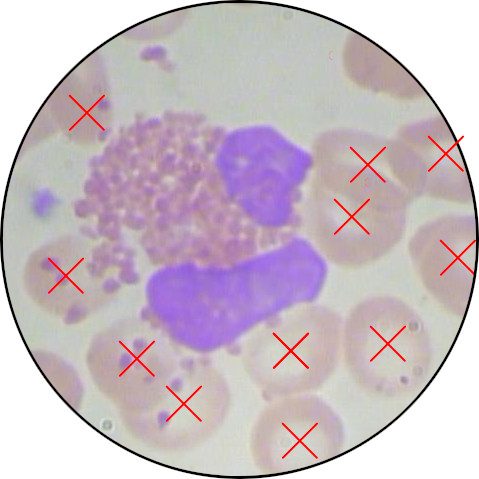
\includegraphics[width=6em]{img/cells_cropped_labeled_edge.png}
                %         \raisebox{2.5em}{$\qquad\xrightarrow{\quad \large\text{rotate}\quad}\qquad$}
                %         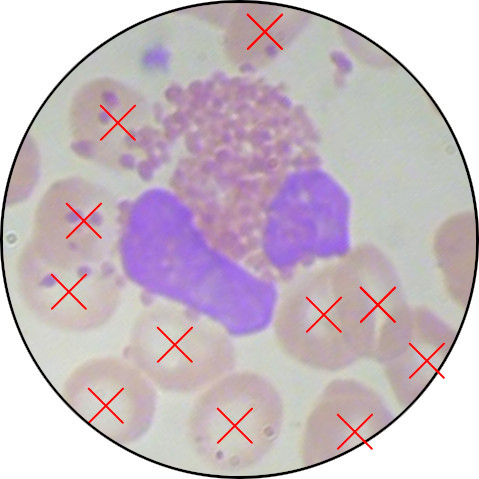
\includegraphics[width=6em]{img/cells_rotated_labeled_edge.png}
                %     \end{center}
                % \end{alertblock}
                % \medskip
                \begin{alertblock}{\huge{Equivariance}}
                    %\begin{block}{Subheading B}
                    %\rmfamily{
                        \begin{itemize}
                          % \item A model is equivariant if when the input is transformed the output transforms “accordingly”
                            \item{Many machine learning problems have an inherent symmetry}
                            \item Equivariant neural networks build the symmetries of the problem into the network architecture
                            \item A network is equivariant with respect to a symmetry group $ G $ iff \[ \mathcal{N}(T_g\, x)= T'_g\, \mathcal{N}(x)\qquad  \forall g\in G \]
                            %\item Vary useful attribute for tasks where the model output should transform in a predictable way to a group of known transformations. A task where this is suitable is semantic segmentation.
                            \item Widely used in applications such as quantum chemistry, medical imaging, \dots
                            \item Equivariant networks require a specialized architecture
                            \item Equivariance is guaranteed to hold exactly

                        \end{itemize}

                    %}

                    %\end{block}
                    %\medskip
                    %\begin{block}{Subheading C}
                    %    \rmfamily{
                    %        \begin{enumerate}
                    %            \item Step 1
                    %            \item Step 2
                    %            \item Step 3 (The important one!)
                    %        \end{enumerate}
                    %    }
                    %
                    %\end{block}

                \end{alertblock}
                \medskip
                \begin{alertblock}{\huge{Data augmentation}}
                    %\begin{block}{Something}
                    %    Text w/o rm family.
                    %\end{block}
                    %\rmfamily{
                        \begin{itemize}
                            \item Enlarge training set by adding transformed data points
                            %\item Useful when one wants to have certain transformations represented in the dataset
                            \item Increases training time% due to more data for the model to work through
                            %\item Requires more memory for the additional data
                            \item No need for specialized architecture, thus easy to implement
                            \item No guarantee for exact equivariance
                        \end{itemize}
                    %}
                \end{alertblock}
                %\vspace{0.37in}
                \medskip
                %\begin{alertblock}{\huge{Model tasks}}
                %    \rmfamily{%
                %        In this work we study semantic segmentation for single and multiple digit spherical MNIST images as well as classification for single digit spherical MNIST images.
                %    }
                %\end{alertblock}
                %\medskip
                \begin{alertblock}{\huge{Dataset}}
                    \begin{itemize}
                        \item MNIST digits projected onto the sphere with classification labels and segmentation masks
                    \end{itemize}
                    {\sffamily
                    \begin{figure}
                        \newcommand{\dualfigscale}{0.25}
                        \centering
                        \hfill{}
                        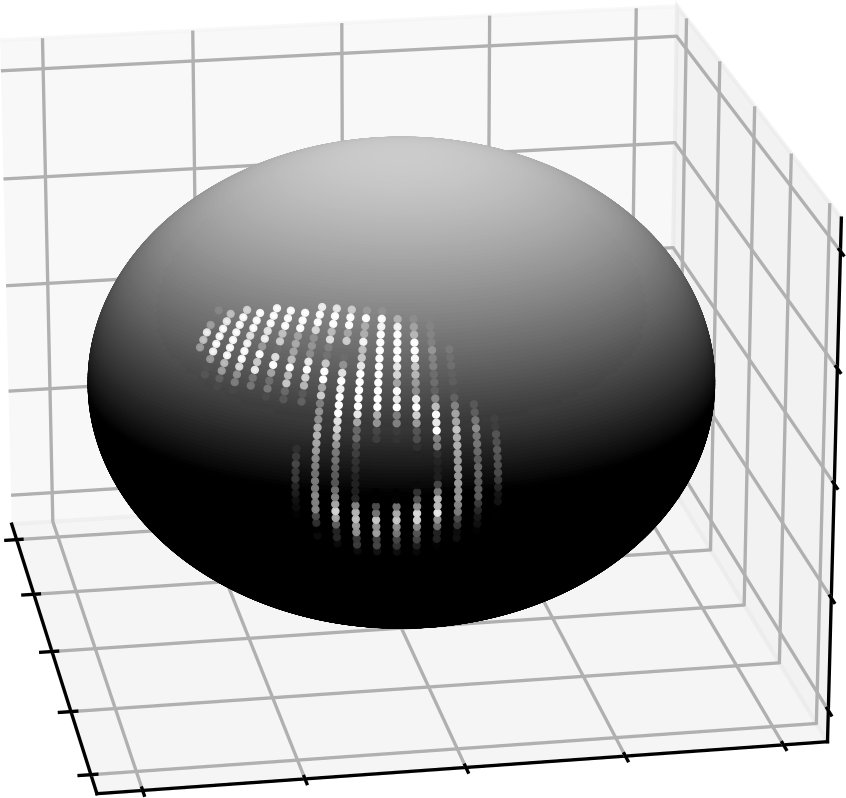
\includegraphics[width=\dualfigscale\columnwidth]{img/spherical_MNIST_input.png}
                        \hfill{}
                        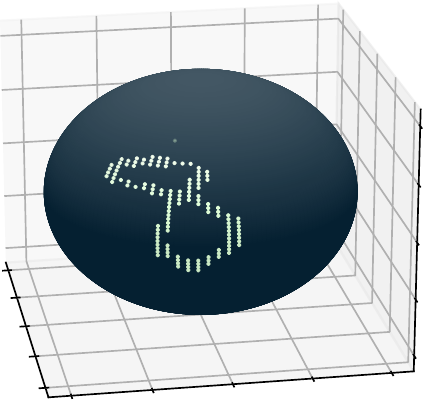
\includegraphics[width=\dualfigscale\columnwidth]{img/spherical_MNIST_label.png}
                        \hfill{}
                        %\caption{Sample from the spherical MNIST dataset used for semantic segmentation. Left: input data. Right: segmentation mask.}
                        %\vspace*{-0.5cm}
                        %\label{fig:sphericalMNIST}
                    \end{figure}
                    }
                \end{alertblock}

                %\medskip
                %\begin{alertblock}{}
                %    \begin{figure}
                %        \centering
                %        
\includegraphics[width=0.4\textwidth]{img/paper_qrcode.png}
                %    \end{figure}
                %\end{alertblock}
                \vfill
                \noindent\footnotesize{Poster presented at ICML-2022 in Baltimore.}
            \end{column}

            %-----------------------------------------------------------
            % Left/Mid Spacer
            %-----------------------------------------------------------
            \begin{column}{\sepwid}
            \end{column}

            %-----------------------------------------------------------
            % Middle Column
            %-----------------------------------------------------------

            \begin{column}{\twocolwid}
                \vspace{-.6in}
                %\begin{columns}[t, totalwidth=\midwid]
                %\begin{column}{\twocolwid}

                % \vspace{-.8in}

                \begin{alertblock}{\huge{Research question}}
                    %Investigating to what degree complex symmetries and transformations can be learnt by simple models through data augmentation compared to models specifically designed for that task.
                    \centering\LARGE
                    Analyze trade-off between data augmentation and equivariance for invariant and equivariant tasks.
                \end{alertblock}
                \medskip
                \begin{alertblock}{\huge{Key takeaway}}
                    \centering
                    \setlength{\columnsep}{60pt}
                    \begin{multicols}{2}
                        %\setlength\columnsep{50pt}
                        For equivariant tasks, the performance of non-equivariant networks trained with data augmentation saturates well below the performance of much smaller equivariant models.

                        \columnbreak

                        For invariant tasks, the performance of larger non-equivariant networks trained with data augmentation can reach the performance of equivariant networks, although the non-equivariant networks take longer to train.
                    \end{multicols}
                    %{ For invariant tasks, the performance of larger non-equivariant networks trained with data augmentation can reach the performance of equivariant networks, although the non-equivariant networks take longer to train.
                    %    %equivariant networks outperforms data augmentation by a large margin even for much larger models
                    %}
                    %%1. equiv tasks: equivariant net > ord+data aug
                    %2. inv task: data aug can compete
                    %3. longer train time for data aug
                \end{alertblock}
                \bigskip
                \begin{alertblock}{\huge{Main results}}
                    \vspace{1cm}
                    \begin{columns}[t, totalwidth=.95\twocolwid]
                        \begin{column}{.92\twocolwid}
                            \vspace{-.7in}
                            \begin{block}{\hphantom{sdfgi}\Large Performance}
                                \begin{center}
                                  \hspace*{2.5em}Numbers in model names refer to the number of trainable parameters
                                \end{center}
                                \begin{center}
                                    \begin{figure}[!ht]
                                        %\begin{center}
                                            %\includegraphics[width = .97\twocolwid]{graeco-latin-square}
                                            \hfill{}
                                            {% This file was created with tikzplotlib v0.9.12.
%\pgfplotsset{y tick label style={font=\bfseries}}% modifies ‘every y tick label'
\begin{tikzpicture}[scale=\figscaleGraph, every node/.style={scale={\figscaleGraph*\textscaleGraph}}]

    \definecolor{color0}{rgb}{0.917647058823529,0.917647058823529,0.949019607843137}
    \definecolor{color1}{rgb}{0.505882352941176,0.447058823529412,0.698039215686274}
    \definecolor{color2}{rgb}{0.298039215686275,0.447058823529412,0.690196078431373}
    \definecolor{color3}{rgb}{0.333333333333333,0.658823529411765,0.407843137254902}
    \definecolor{color4}{rgb}{0.768627450980392,0.305882352941176,0.32156862745098}

    \begin{axis}[
        %height=5.5cm,
        width=\figw,
        axis background/.style={fill=color0},
        axis line style={white},
        legend cell align={left},
        legend style={
            fill opacity=0.8,
            draw opacity=1,
            text opacity=1,
            at={\graphlegendpos},
            anchor=south east,
            draw=none,
            fill=color0,
            %mark size=100pt
        },
        legend image post style={scale=2.5}, % rescales the markers in the legend
        tick align=outside,
        tick pos=left,
        title={Semantic segmentation},
        title style={at={\titlepos}},
        x grid style={white},
        xlabel style={yshift=\xlabelyshift},
        xlabel={Number of training images},
        xmajorgrids,
        xmin=-0.06, xmax=1.26,
        xtick style={color=white!85!black, font=\tiny},
        xtick={0,0.2,0.4,0.6,0.8,1,1.2},
        xticklabels={0,200k,400k,600k,800k,1.0M,1.2M},
        y grid style={white},
        ylabel style={yshift=\ylabelyshift},
        ylabel={Non-background IoU},
        ymajorgrids,
        ymin=0, ymax=100,
        ytick style={color=white!85!black, font=\tiny},
        %yticklabel={%
        %    %\scriptsize
        %    \normalsize % Sets font size
        %    \ifdim\tick pt<0pt % a TeX \if -- see TeX Book, i.e. if \tick is negative, has to use a dimensional comparison due to \ifdim hence “\tick pt”
        %        \pgfmathparse{-10*\tick}%
        %        $-\nicefrac{\pgfmathprintnumber{\pgfmathresult}}{10}$%
        %    \else
        %        \ifdim\tick pt=0pt  % if \tick is 0 don't do anything
        %        \else
        %            \pgfmathparse{10*\tick}%
        %            $\nicefrac{\pgfmathprintnumber{\pgfmathresult}}{10}$%
        %        \fi
        %    \fi
        %},
        %yticklabel={\tick}, # Too many decimals
        %yticklabel = {$\pgfmathprintnumber[precision=0]{\tick}$},  % Good number of decimals, wrong font
        yticklabel = {\pgfmathsfprintnumber[precision=0]{\tick}},  % THIS WORKS
        %yticklabel style={
        %    font=\bfseries,%\fontfamily{lmss}\selectfont,
        %    yshift=\ylabelyshift
        %},
        %yticklabel style={/pgf/number format/.cd,frac,
        %     frac TeX=\nicefrac,frac whole=false,frac denom=10},
        ]
        \path [
            draw=color1,
            %line width=0.7pt,
            line width=\graphlinewidth{}pt,
            dash pattern=on 6.475pt off 2.8pt
            ]
        (axis cs:0,79.0172031795914)
        --(axis cs:1.2,79.0172031795914);

        \addplot [
            %very thick,
            line width=\graphlinewidth{}pt,
            color1,
            mark=*,
            mark size=3.5,
            mark options={solid}
            ]
        table {%
            0.01 73.6672228087486
            0.02 76.2396656837297
            0.03 75.9440592307601
            0.04 77.0006140071276
            0.05 78.0121633327085
            0.06 78.2821354107209
            0.08 78.6005328484791
            0.1 78.3440466722201
            0.1 78.7591833919464
            0.12 78.6653772927548
            0.24 79.0172031795914
        };
        \addlegendentry{\color{black}204k S2CNN}
        \addplot [
            %very thick,
            line width=\graphlinewidth{}pt,
            color2,
            mark=+,
            mark size=3.5,
            mark options={solid}
            ]
        table {%
            0.01 33.9979413230564
            0.02 35.2098953469084
            0.03 36.6968152116464
            0.04 36.3691463001431
            0.05 36.8220698817118
            0.06 37.2769826449922
            0.08 40.2635431161527
            0.1 40.2390027250844
            0.12 47.0656347978214
            0.24 49.6463416406717
            0.6 49.4607500191341
            1.2 49.3667478680225
        };
        \addlegendentry{\color{black}218k CNN}
        \addplot [
            %very thick,
            line width=\graphlinewidth{}pt,
            color3,
            mark=+,
            mark size=3.5,
            mark options={solid}
            ]
        table {%
            0.01 40.5212931678065
            0.02 41.377917930675
            0.03 43.251758735901
            0.04 42.6359169287997
            0.05 44.2412785935146
            0.06 44.5472077883157
            0.08 49.1886897951291
            0.1 48.7415286074443
            0.12 55.0321060520411
            0.24 58.6775255398797
            0.6 60.5768117291
            1.2 61.4187406860649
        };
        \addlegendentry{\color{black}1M CNN}
        \addplot [
            %very thick,
            line width=\graphlinewidth{}pt,
            color4,
            mark=+,
            mark size=3.5,
            mark options={solid}
            ]
        table {%
            0.01 39.8560257098186
            0.02 39.2542836381079
            0.03 40.2511386267728
            0.04 40.9095744779148
            0.05 43.239519380981
            0.06 42.5646759801113
            0.08 46.8256498871211
            0.1 47.1734684919231
            0.12 54.0339057646098
            0.24 57.5987507390389
            0.6 56.9030047900288
            1.2 59.1977968380171
        };
        \addlegendentry{\color{black}5.5M CNN}
    \end{axis}

\end{tikzpicture}
}%
                                            \hfill{}%
                                            {% This file was created with tikzplotlib v0.9.12.
\tikzset{discont/.style={decoration={zigzag,segment length=12pt, amplitude=4pt},decorate}}
\begin{tikzpicture}[scale=\figscaleGraph, every node/.style={scale={\figscaleGraph*\textscaleGraph}}, font={\sffamily\selectfont}]

    \definecolor{color0}{rgb}{0.917647058823529,0.917647058823529,0.949019607843137}
    \definecolor{color1}{rgb}{0.505882352941176,0.447058823529412,0.698039215686274}
    \definecolor{color2}{rgb}{0.298039215686275,0.447058823529412,0.690196078431373}
    \definecolor{color3}{rgb}{0.333333333333333,0.658823529411765,0.407843137254902}
    \definecolor{color4}{rgb}{0.768627450980392,0.305882352941176,0.32156862745098}

    \begin{axis}[
        %height=5.5cm,
        width=\figw,
        axis background/.style={fill=color0},
        axis line style={white},
        legend cell align={left},
        legend style={
            fill opacity=0.8,
            draw opacity=1,
            text opacity=1,
            %at={(0.97,0.03)},
            at={\graphlegendpos},
            anchor=south east,
            draw=none,
            fill=color0
        },
        legend image post style={scale=2.5}, % rescales the markers in the legend
        tick align=outside,
        tick pos=left,
        x grid style={white},
        title={Classification},
        title style={at={\titlepos}},
        xlabel={Number of training images},
        xlabel style={yshift=\xlabelyshift},
        xmajorgrids,
        xmin=-60, xmax=1260,
        xtick style={color=white!85!black},
        xtick={0,200,400,600,800,1000,1200},
        xticklabels={0,200k,400k,600k,800k,1.0M,1.2M},
        y grid style={white},
        ylabel={Test accuracy},
        ylabel style={yshift=\ylabelyshift},
        ymajorgrids,
        ymin=80, ymax=100,
        ytick style={color=white!85!black, font={\sffamily\selectfont}},
        %enlargelimits=false,
        %axis y discontinuity=crunch,
        ]
        \path [draw=color1, line width=\graphlinewidth{}pt, dash pattern=on 6.475pt off 2.8pt]
        (axis cs:0,98.58)
        --(axis cs:1200,98.58);

        \addplot [
            %very thick,
            line width=\graphlinewidth{}pt,
            color1,
            mark=*,
            mark size=3.5,
            mark options={solid}
            ]
        table {%
            10 91.81
            20 96.01
            30 97.26
            40 96.61
            50 97.54
            60 97.64
            100 98.5
            120 98.47
            240 98.58
        };
        \addlegendentry{150k S2CNN}
        \addplot [
            %very thick,
            line width=\graphlinewidth{}pt,
            color2,
            mark=+,
            mark size=3.5,
            mark options={solid}
            ]
        table {%
            10 85.16
            20 86.77
            30 87.26
            40 87.41
            50 90.03
            60 89.46
            80 91.48
            100 91.5
            120 94.43
            240 95.65
            600 95.86
            1200 97.14
        };
        \addlegendentry{114k CNN}
        \addplot [
            %very thick,
            line width=\graphlinewidth{}pt,
            color3,
            mark=+,
            mark size=3.5,
            mark options={solid}
            ]
        table {%
            10 86.33
            20 87.07
            30 88.08
            40 89.78
            50 91.16
            60 91.81
            80 93.15
            100 94.01
            120 95.5
            240 97.05
            600 97.36
            1200 98.01
        };
        \addlegendentry{0.5M CNN}
        \addplot [
            %very thick,
            line width=\graphlinewidth{}pt,
            color4,
            mark=+,
            mark size=3.5,
            mark options={solid}
            ]
        table {%
            10 86.63
            20 86.42
            30 88.15
            40 89.02
            50 91.93
            60 92.21
            80 93.13
            100 94.01
            120 95.44
            240 96.59
            600 97.49
            1200 98.3
        };
        \addlegendentry{2.5M CNN}
    \end{axis}

\end{tikzpicture}
}%
                                            \hfill{}%
                                            \hspace{1cm}
                                        %\end{center}
                                        %\caption{\rmfamily{\textit{Non-equivariant performance saturation for segmentation}. Left: For classification of spherical MNIST as in Figure~\ref{fig:spherical_classification}, the non-equivariant models reach the test accuracy of the equivariant models for very large amounts of data augmentation. Right: For semantic segmentation of one-digit spherical MNIST as in Figure~\ref{fig:data_augm_1_digit}, the non-background IoU of the non-equivariant models saturates well below the performance of the equivariant model even for moderately high amounts of data augmentation.}}
                                    \end{figure}
                                \end{center}


                            \end{block}
                            \medskip
                            \begin{block}{\hphantom{sdfgi}\Large Throughput and training times}
                                %\begin{table}[t]
                                %    %\caption{Runtime latency and throughput for the equivariant semantic segmentation model (204k S2CNN in Appendix Table~\ref{tab:equiv_models}) on an Nvidia T4 16GB GPU. Latency measures the time of a forward pass through the model on the GPU, throughput is the corresponding number of samples per second given the batch size. The larger batch size is chosen to maximize the throughput for the T4.}
                                %    \label{tab:spherical_performance}
                                %    \begin{tabular}{lll}
                                    %        Batch size & Latency (ms)  & Throughput (N/s) \\
                                    %        \hline
                                    %        1          & $111\pm{0.6}$ & $9.0\pm{0.04}$   \\
                                    %        7          & $479\pm{2.2}$ & $14.6\pm{0.07}$
                                    %    \end{tabular}
                                %\end{table}

                                %\begin{table}[t]
                                %    %\caption{Runtime latency and throughput for non-equivariant CNN model (200k CNN in Appendix Table~\ref{tab:equiv_models}) on an Nvidia T4 16GB GPU. Latency measures the time of a forward pass through the model on the GPU, throughput is the corresponding number of samples per second given the batch size. The larger batch size is chosen to maximize the throughput for the T4.}
                                %    \label{tab:CNN_performance}
                                %    \begin{tabular}{lll}
                                    %        Batch size & Latency (ms)  & Throughput (N/s) \\
                                    %        \hline
                                    %        1 & $5.93 \pm{0.24} $ &  $169 \pm{5.8}$ \\
                                    %        60 & $87.98 \pm{0.17}$ & $682 \pm{1.3}$
                                    %    \end{tabular}
                                %\end{table}
                                \setlength{\columnsep}{60pt}
                                \begin{multicols}{2}
                                    %\begin{table}
                                    \centering
                                    Due to the specialized architecture the equivariant model has much higher latency at similar parameter counts than the non-equivariant models.\\[1em]
                                    \leavevmode\\
                                    {\setlength{\tabcolsep}{30pt}
                                    \begin{tabular}{l@{}S@{}@{}S@{}}
                                        \toprule
                                        Model & {\hspace{1em}Latency (ms)\hspace{1em}}  & {Throughput (N/s)} \\\midrule
                                        204k S2CNN     & 111+-0.6 & 9.0+-0.04   \\
                                        200k CNN     & 5.93+-0.24  &  169+-5.8 \\
                                        \bottomrule
                                    \end{tabular}
                                    %\end{table}

                                    \columnbreak

                                    %\begin{table}[t]
                                    \centering
                                    %\caption{Training times for the S2CNN classification model and non-equivariant CNN model at matched accuracy on rotated spherical images. The S2CNN model is trained on non-rotated images whereas the CNN is trained on an augmented dataset with rotated images. A single Nvidia T4 16GB was used for training.}
                                    %\label{tab:classification_training_times}
                                    At matched accuracy the total training time for the non-equivariant model trained with data augmentation is much higher than the training time for the equivariant model trained without data augmentation.\\[1em]
                                    \begin{tabular}{lcc}
                                        \toprule
                                        Model      & Accuracy & Training time \\\midrule
                                        150k S2CNN & 97.64\%    & 15h           \\
                                        5M CNN     & 97.49\%    & 26h          \\
                                        \bottomrule
                                    \end{tabular}}
                                    %\end{table}
                                \end{multicols}


                            \end{block}


                            %\rmfamily{\small{\color{dblue}Figure 1: \color{black} \textit{Non-equivariant performance saturation for segmentation}. Left: For classification of spherical MNIST as in Figure~\ref{fig:spherical_classification}, the non-equivariant models reach the test accuracy of the equivariant models for very large amounts of data augmentation. Right: For semantic segmentation of one-digit spherical MNIST as in Figure~\ref{fig:data_augm_1_digit}, the non-background IoU of the non-equivariant models saturates well below the performance of the equivariant model even for moderately high amounts of data augmentation.}}\\

                        \end{column}
                    \end{columns}
                %\begin{block}{Another Subheading!}
                %    Originally there were 5 pictures here, but since we've already used the subfigure command, I'll just say you could put words here, with one or two columns.
                %
                %    \begin{columns}[t, totalwidth=.95\twocolwid]
                %        \begin{column}{.92\onecolwid}
                %            words.
                %        \end{column}
                %        \begin{column}{.92\onecolwid}
                %            words.
                %        \end{column}
                %    \end{columns}
                %\end{block}

            \end{alertblock}



        \end{column}

        %-----------------------------------------------------------
        % Mid/Right Spacer
        %-----------------------------------------------------------

        \begin{column}{\sepwid}
        \end{column}			% empty spacer column

        %-----------------------------------------------------------
        % Right Column
        %-----------------------------------------------------------
        \begin{column}{\onecolwid}
            \vspace{-.6in}

            \begin{alertblock}{\huge{Further results}}

                %\rmfamily{words.}. \\

                %\justifying



                %\begin{figure}[!ht]
                %    \begin{center}
                %        \subfigure{
                %            \scalebox{1.0}{\includegraphics[width = .45\onecolwid,height=.39375\onecolwid]{graeco-latin-square}}}
                %        \subfigure{
                %            \scalebox{1.0}{\includegraphics[width = .45\onecolwid,height=.39375\onecolwid]{graeco-latin-square}}}
                %    \end{center}
                %\end{figure}
                %\rmfamily{\small{\color{dblue}Figure 4: \color{black}  some pictures!}}\\

                %And now some words about this picture. Picture picture picture picture picture words.

                \begin{block}{\Large Rotated vs non-rotated test images}
                    %\rmfamily{
                        When training is performed only on unrotated images, the non-equivariant models outperform the equivariant models on unrotated test data. On rotated test data, the non-equivariant performance deteriorates whereas the equivariant performance is unaffected.
                        \begin{figure}[h]
                            \centering
                            % \includegraphics[width=0.49\textwidth]{imgs/spherical_data_augmentation_non_rot_non_rot_eval.pdf}
                            \resizebox{0.49\textwidth}{!}{% This file was created with tikzplotlib v0.9.12.
\begin{tikzpicture}

    \definecolor{color0}{rgb}{0.917647058823529,0.917647058823529,0.949019607843137}
    \definecolor{color1}{rgb}{0.505882352941176,0.447058823529412,0.698039215686274}
    \definecolor{color2}{rgb}{0.298039215686275,0.447058823529412,0.690196078431373}
    \definecolor{color3}{rgb}{0.333333333333333,0.658823529411765,0.407843137254902}
    \definecolor{color4}{rgb}{0.768627450980392,0.305882352941176,0.32156862745098}

    \begin{axis}[
        width=\smallfigw,
        axis background/.style={fill=color0},
        axis line style={white},
        legend cell align={left},
        legend style={
            fill opacity=0.8,
            draw opacity=1,
            text opacity=1,
            at={(0.97,0.03)},
            anchor=south east,
            draw=none,
            fill=color0
        },
        legend image post style={scale=\smalllegendscale}, % rescales the markers in the legend
        tick align=outside,
        tick pos=left,
        %title={Training on Unrotated Images},
        x grid style={white},
        xlabel={Number of unrotated training images},
        xmajorgrids,
        xmin=-1.5, xmax=251.5,
        xtick style={color=white!15!black},
        xtick={0,50,100,150,200,250},
        xticklabels={0,50k,100k,150k,200k,250k},
        y grid style={white},
        ylabel={mIoU on Unrotated Images},
        ymajorgrids,
        ymin=0, ymax=100,
        ytick style={color=white!15!black}
        ]
        \addplot [
            %very thick,
            line width=\smallgraphlinewidth{}pt,
            color1,
            mark=*,
            mark size=\smallmarksize,
            mark options={solid}
            ]
        table {%
            10 74.2677050380129
            20 76.8594136096554
            30 77.6652588021171
            40 77.4544267995054
            50 78.5149509435184
            60 78.9408037774072
            80 79.2532051489549
            100 79.3389975715341
            120 79.6200572759775
            240 79.8134576137201
        };
        \addlegendentry{204k S2CNN}
        \addplot [
            %very thick,
            line width=\smallgraphlinewidth{}pt,
            color2,
            mark=+,
            mark size=\smallmarksize,
            mark options={solid}
            ]
        table {%
            10 73.58010400801
            20 78.7023771991111
            30 78.9041138752722
            40 79.3057521588921
            50 80.5108672546465
            60 80.2258178334838
            80 80.7878977638898
            100 81.4627986946612
            120 82.0625219880998
            240 82.4408405267292
        };
        \addlegendentry{218k CNN}
        \addplot [
            %very thick,
            line width=\smallgraphlinewidth{}pt,
            color3,
            mark=+,
            mark size=\smallmarksize,
            mark options={solid}
            ]
        table {%
            10 78.2265176796211
            20 80.535194868353
            30 82.0018308336076
            40 81.6911872451438
            50 81.2831222653486
            60 82.2505874229562
            80 82.7425805840175
            100 80.9219300755188
            120 82.7111695574602
            240 81.9464730390086
        };
        \addlegendentry{1M CNN}
        \addplot [
            %very thick,
            line width=\smallgraphlinewidth{}pt,
            color4,
            mark=+,
            mark size=\smallmarksize,
            mark options={solid}
            ]
        table {%
            10 78.0618706094855
            20 81.3463741541022
            30 83.3847572361571
            40 84.2081055815584
            50 84.6111215789895
            60 84.4535715293519
            80 85.2798405602758
            100 85.8347079643411
            120 86.1351850568458
            240 87.1462695739364
        };
        \addlegendentry{5.5M CNN}
    \end{axis}

\end{tikzpicture}
}
                            \hfill
                            % \includegraphics[width=0.49\textwidth]{imgs/spherical_data_augmentation_non_rot_rot_eval.pdf}
                            \resizebox{0.49\textwidth}{!}{% This file was created with tikzplotlib v0.9.12.
\begin{tikzpicture}

    \definecolor{color0}{rgb}{0.917647058823529,0.917647058823529,0.949019607843137}
    \definecolor{color1}{rgb}{0.505882352941176,0.447058823529412,0.698039215686274}
    \definecolor{color2}{rgb}{0.298039215686275,0.447058823529412,0.690196078431373}
    \definecolor{color3}{rgb}{0.333333333333333,0.658823529411765,0.407843137254902}
    \definecolor{color4}{rgb}{0.768627450980392,0.305882352941176,0.32156862745098}

    \begin{axis}[
        width=\smallfigw,
        axis background/.style={fill=color0},
        axis line style={white},
        legend cell align={left},
        legend style={
            fill opacity=0.8,
            draw opacity=1,
            text opacity=1,
            at={(0.91,0.5)},
            anchor=east,
            draw=none,
            fill=color0
        },
        legend image post style={scale=\smalllegendscale}, % rescales the markers in the legend
        legend style={at={(0.98,0.65)}, anchor=north east},
        tick align=outside,
        tick pos=left,
        %title={Training on Unrotated Images},
        x grid style={white},
        xlabel={Number of unrotated training images},
        xmajorgrids,
        xmin=-1.5, xmax=251.5,
        xtick style={color=white!15!black},
        xtick={0,50,100,150,200,250},
        xticklabels={0,50k,100k,150k,200k,250k},
        y grid style={white},
        ylabel={mIoU on Rotated Images},
        ymajorgrids,
        ymin=0, ymax=100,
        ytick style={color=white!15!black}
        ]
        \addplot [
            %very thick,
            line width=\smallgraphlinewidth{}pt,
            color1,
            mark=*,
            mark size=\smallmarksize,
            mark options={solid}
            ]
        table {%
            10 75.1587116491286
            20 77.2851588144363
            30 77.8402581084608
            40 77.7334137544592
            50 78.4878156072444
            60 78.5875963391494
            80 78.5976902440102
            100 78.7177660313421
            120 78.7853338790605
            240 78.9656905254994
        };
        \addlegendentry{204k S2CNN}
        \addplot [
            %very thick,
            line width=\smallgraphlinewidth{}pt,
            color2,
            mark=+,
            mark size=\smallmarksize,
            mark options={solid}
            ]
        table {%
            10 15.4105544086955
            20 11.1467325010807
            30 8.87570742592795
            40 11.5564898197759
            50 10.3677151806773
            60 13.9558447331002
            80 11.2701381964532
            100 13.9038172230294
            120 8.72533194444059
            240 13.4127458878852
        };
        \addlegendentry{218k CNN}
        \addplot [
            %very thick,
            line width=\smallgraphlinewidth{}pt,
            color3,
            mark=+,
            mark size=\smallmarksize,
            mark options={solid}
            ]
        table {%
            10 15.5062010399999
            20 9.55727127915249
            30 10.7656904274824
            40 10.9923507777807
            50 11.0679791346708
            60 14.6015120060682
            80 10.749363031772
            100 14.4085376092666
            120 7.95947345375563
            240 13.3799775522978
        };
        \addlegendentry{1M CNN}
        \addplot [
            %very thick,
            line width=\smallgraphlinewidth{}pt,
            color4,
            mark=+,
            mark size=\smallmarksize,
            mark options={solid}
            ]
        table {%
            10 13.2053186386201
            20 10.14357604628
            30 9.75132015740805
            40 11.0343348734973
            50 9.92196461811875
            60 13.1360583893131
            80 9.52646708318885
            100 13.4541821036274
            120 9.22203602195639
            240 15.227933881533
        };
        \addlegendentry{5.5M CNN}
    \end{axis}

\end{tikzpicture}
}
                            %\caption{\textit{Training on Unrotated Images}. Performance of equivariant and non-equivariant models in semantic segmentation for various amounts of data augmentation for models trained on unrotated data with one digit. Performance  is  measured  in terms of mIoU for the non-background classes. Left: evaluated on unrotated test data. Right: evaluated on rotated test data.}
                            %\label{fig:data_augm_non_rot}
                        \end{figure}
                    %}
                \end{block}
                \medskip
                \begin{block}{\Large Multiple digits}
                    Similar results hold for semantic segmentation with four digits projected onto the sphere.
                    \begin{figure}
                        \centering
                        % \includegraphics[width=0.9\columnwidth]{imgs/spherical_data_augmentation_4_digits.pdf}
                        \hspace{2em}
                        \raisebox{1.75em}{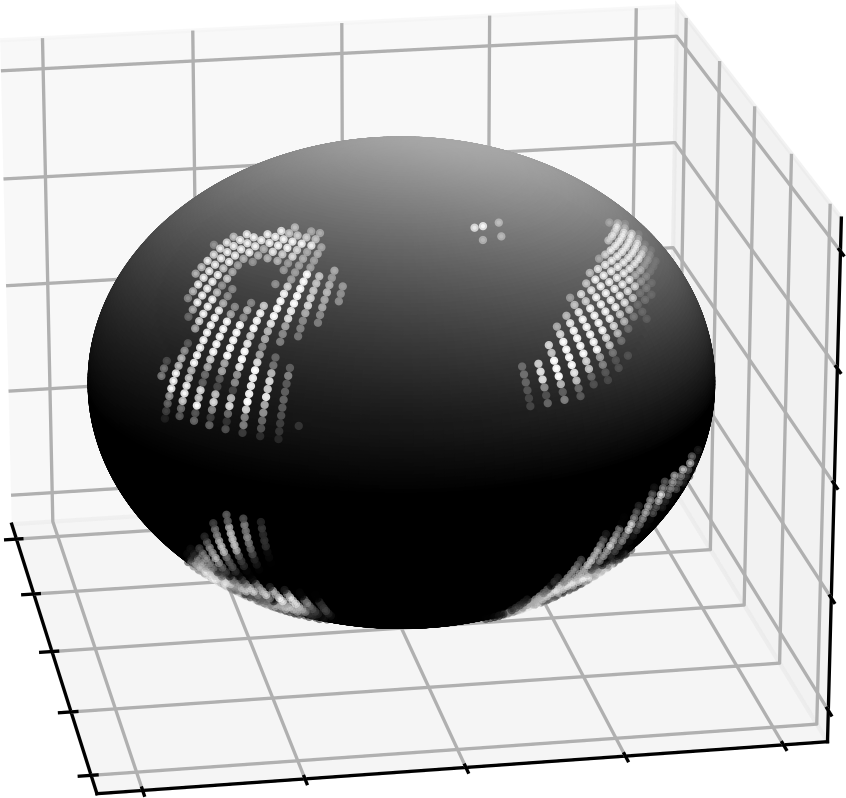
\includegraphics[width=0.35\columnwidth]{img/spherical_MNIST_input_4_digits.png}}
                        \hspace{2em}
                        \resizebox{0.49\textwidth}{!}{% This file was created with tikzplotlib v0.9.12.
\begin{tikzpicture}

    \definecolor{color0}{rgb}{0.917647058823529,0.917647058823529,0.949019607843137}
    \definecolor{color1}{rgb}{0.505882352941176,0.447058823529412,0.698039215686274}
    \definecolor{color2}{rgb}{0.298039215686275,0.447058823529412,0.690196078431373}
    \definecolor{color3}{rgb}{0.333333333333333,0.658823529411765,0.407843137254902}
    \definecolor{color4}{rgb}{0.768627450980392,0.305882352941176,0.32156862745098}

    %\begin{axis}[
    %    axis background/.style={fill=color0},
    %    axis line style={white},
    %    legend cell align={left},
    %    legend style={
    %        fill opacity=0.8,
    %        draw opacity=1,
    %        text opacity=1,
    %        at={(0.97,0.03)},
    %        anchor=south east,
    %        draw=none,
    %        fill=color0
    %    },
    %    tick align=outside,
    %    tick pos=left,
    %    %title={Segmentation on four digit Spherical MNIST},
    %    x grid style={white},
    %    xlabel={Number of training images},
    %    xmajorgrids,
    %    xmin=-1.5, xmax=251.5,
    %    xtick style={color=white!15!black},
    %    xtick={0,50,100,150,200,250},
    %    xticklabels={0,50k,100k,150k,200k,250k},
    %    y grid style={white},
    %    ylabel={mIoU (non-background)},
    %    ymajorgrids,
    %    ymin=0, ymax=100,
    %    ytick style={color=white!15!black}
    %    ]
    \begin{axis}[
        width=\smallfigw,
        axis background/.style={fill=color0},
        axis line style={white},
        legend cell align={left},
        legend style={
            fill opacity=0.8,
            draw opacity=1,
            text opacity=1,
            at={(0.97,0.03)},
            anchor=south east,
            draw=none,
            fill=color0
        },
        legend image post style={scale=\smalllegendscale}, % rescales the markers in the legend
        tick align=outside,
        tick pos=left,
        %title={Training on Unrotated Images},
        x grid style={white},
        xlabel={Number of unrotated training images},
        xmajorgrids,
        xmin=-1.5, xmax=251.5,
        xtick style={color=white!15!black},
        xtick={0,50,100,150,200,250},
        xticklabels={0,50k,100k,150k,200k,250k},
        y grid style={white},
        ylabel={mIoU on Unrotated Images},
        ymajorgrids,
        yticklabel = {\pgfmathsfprintnumber[precision=0]{\tick}},  % THIS WORKS
        ymin=0, ymax=100,
        ytick style={color=white!15!black}
        ]
        \addplot [very thick, color1, mark=*, mark size=3.5, mark options={solid}]
        table {%
            10 73.6574362848322
            20 76.0395833736555
            30 76.7890055815408
            40 77.5328788714405
            50 77.020082794026
            60 77.8381367155123
            80 78.2197165462477
            100 77.9684623342617
            120 78.1636630549863
            240 78.3261777832088
        };
        \addlegendentry{204k S2CNN}
        \addplot [very thick, color2, mark=+, mark size=3.5, mark options={solid}]
        table {%
            10 32.7623520492889
            20 39.785570381459
            30 45.6672944820466
            40 43.6034531633931
            50 52.9660619529629
            60 47.3842111139795
            80 50.7463134189105
            100 46.5693888014821
            120 54.5243203801985
            240 55.2213802508576
        };
        \addlegendentry{218k CNN}
        \addplot [very thick, color3, mark=+, mark size=3.5, mark options={solid}]
        table {%
            10 35.9387544826403
            20 46.3409641066674
            30 50.8084672150865
            40 48.5435259540383
            50 58.9691012445147
            60 54.1634577116196
            80 59.2485369254248
            100 55.0810140666171
            120 61.8213733749629
            240 62.4269677407072
        };
        \addlegendentry{1M CNN}
        \addplot [very thick, color4, mark=+, mark size=3.5, mark options={solid}]
        table {%
            10 31.7295263691858
            20 41.5629787039001
            30 47.0335572651033
            40 44.6008543255815
            50 56.2212101792903
            60 50.878548185644
            80 57.4930188112352
            100 52.2904181758365
            120 60.3875023574351
            240 61.5921850677986
        };
        \addlegendentry{5.5M CNN}
    \end{axis}

\end{tikzpicture}
}
                        

                        %\caption{\textit{Segmentation on four digit Spherical MNIST}. Performance of equivariant and non-equivariant models in semantic segmentation for various amounts of data augmentation as in Figure~\ref{fig:data_augm_1_digit}, but with four digits projected onto the sphere.}
                        %\label{fig:data_augm_4_digits}
                    \end{figure}
                %\begin{figure}[t]
                %    \centering
                %
                %    \hfill
                %    \includegraphics[width=0.4\columnwidth]{imgs/spherical_MNIST_label_4_digits.png}
                %    \caption{Sample from the spherical MNIST dataset with four digits projected onto the sphere. Left: input data. Right: segmentation mask.}
                %    \label{fig:sphericalMNIST_4_digits}
                %\end{figure}
                \end{block}
                \begin{block}{\Large New equivariant S2CNN layer for semantic segmentation}
                    We added a layer to the S2CNN architecture \cite{cohen2018b} reducing feature maps on $ \mathrm{SO}(3) $ to feature maps on $ S^{2} $ for semantic segmentation.\\[2em]
                    \begin{tikzpicture}[scale=\figscale, every node/.style={scale={\figscale*\textscale}}]
    \begin{pgfonlayer}{nodelayer}
        % 		\node [style=none] (0) at (-3.5, 3.25) {};
        % 		\node [style=none] (1) at (-2.5, 3) {};
        % 		\node [style=none] (2) at (-2.5, 4) {};
        \node [style=none] (0) at (-3.5, 3.00) {};
        \node [style=none] (1) at (-2.5, 2.75) {};
        \node [style=none] (2) at (-2.5, 3.75) {};
        \node [style=none] (4) at (-3.25, 5.5) {};
        \node [style=none] (5) at (-0.25, 4.75) {};
        \node [style=none] (6) at (-0.25, 1.75) {};
        \node [style=none] (7) at (-3.25, 2.5) {};
        \node [style=none] (8) at (-3.5, 4.00) {};
        \node [style=none] (9) at (2, 0.75) {};
        \node [style=none] (10) at (2, 5.75) {};
        \node [style=none] (11) at (-3, 7) {};
        \node [style=none] (12) at (-3, 2) {};
        \node [style=none] (13) at (-4.5, 1.25) {};
        \node [style=none] (14) at (-4.5, 2.5) {};
        \node [style=none] (15) at (-3.5, 1.75) {};
        \node [style=none] (16) at (-3.25, 1) {};
        \node [style=none] (18) at (-0.75, 8) {$\mathrm{SO}(3)$  expansion coefficients};
        \node [style=none] (19) at (3.5, 3.25) {};
        \node [style=none] (20) at (8, 3.25) {};
        \node [style=none] (21) at (11.5, 3) {};
        \node [style=none] (22) at (12.5, 2.75) {};
        \node [style=none] (23) at (12.5, 3.75) {};
        \node [style=none] (24) at (11.5, 4) {};
        \node [style=none] (25) at (11.75, 2.25) {};
        \node [style=none] (26) at (12.75, 2) {};
        \node [style=none] (27) at (12.75, 5) {};
        \node [style=none] (28) at (11.75, 5.25) {};
        \node [style=none] (29) at (12, 1.5) {};
        \node [style=none] (30) at (13, 1.25) {};
        \node [style=none] (31) at (13, 6.25) {};
        \node [style=none] (32) at (12, 6.5) {};
        \node [style=none] (33) at (10, 1.25) {};
        \node [style=none] (34) at (10, 3) {};
        \node [style=none] (35) at (11.25, 1.75) {};
        \node [style=none] (36) at (12.5, 8) {$S^2$ expansion coefficients};
        \node [style=none] (37) at (-5.5, 5) {$(\kappa\star f)^\ell_{mn}$};
        \node [style=none] (38) at (-2.25, 5.25) {};
        \node [style=none] (39) at (-1.25, 5) {};
        \node [style=none] (40) at (-2.25, 2.25) {};
        \node [style=none] (41) at (-1.25, 2) {};
        \node [style=none] (42) at (-3.25, 4.5) {};
        \node [style=none] (43) at (-3.25, 3.5) {};
        \node [style=none] (44) at (-0.25, 2.75) {};
        \node [style=none] (45) at (-0.25, 3.75) {};
        \node [style=none] (46) at (1, 1) {};
        \node [style=none] (47) at (0, 1.25) {};
        \node [style=none] (48) at (-1, 1.5) {};
        \node [style=none] (49) at (-2, 1.75) {};
        \node [style=none] (50) at (1, 6) {};
        \node [style=none] (51) at (0, 6.25) {};
        \node [style=none] (52) at (-1, 6.5) {};
        \node [style=none] (53) at (-2, 6.75) {};
        \node [style=none] (54) at (2, 4.75) {};
        \node [style=none] (55) at (2, 3.75) {};
        \node [style=none] (56) at (2, 2.75) {};
        \node [style=none] (57) at (2, 1.75) {};
        \node [style=none] (58) at (-3, 3) {};
        \node [style=none] (59) at (-3, 4) {};
        \node [style=none] (60) at (-3, 5) {};
        \node [style=none] (61) at (-3, 6) {};
        \node [style=none] (62) at (11.75, 3.25) {};
        \node [style=none] (63) at (12.75, 3) {};
        \node [style=none] (64) at (11.75, 4.25) {};
        \node [style=none] (65) at (12.75, 4) {};
        \node [style=none] (66) at (12, 2.5) {};
        \node [style=none] (67) at (13, 2.25) {};
        \node [style=none] (68) at (12, 3.5) {};
        \node [style=none] (69) at (13, 3.25) {};
        \node [style=none] (70) at (12, 4.5) {};
        \node [style=none] (71) at (13, 4.25) {};
        \node [style=none] (72) at (12, 5.5) {};
        \node [style=none] (73) at (13, 5.25) {};
        \node [style=none] (74) at (15, 3.25) {};
        \node [style=none] (75) at (20.5, 3.25) {};
        \node [style=none] (78) at (24.75, 8) {$S^2$};
        \node [style=none] (79) at (24.25, 3.25) {
\includegraphics[width=0.1\textwidth]{img/spherical_mnist_label_sphere_only.png}};
        \node [style=none] (80) at (26.5,4.7) {$f^{\text{final}}$};
    \end{pgfonlayer}
    \begin{pgfonlayer}{edgelayer}
        \draw [style={right_arrow}] (13.center) to node [midway, above] {$\ell$} (15.center);
        \draw [style={right_arrow}] (13.center) to node [midway, left] {$m$} (14.center);
        \draw [style={right_arrow}] (13.center) to node [midway, below] {$n$} (16.center);
        \draw [style={right_arrow}, very thick] (19.center) to node [midway, above] {$\displaystyle\sum_{n=-\ell}^\ell$} (20.center);
        \draw [style={right_arrow}] (33.center) to node [midway, below] {$\ell$} (35.center);
        \draw [style={right_arrow}] (33.center) to node [midway, left] {$m$} (34.center);
        \draw [style={filled_path_edge}] (25.center) to (26.center);
        \draw [style={right_arrow}, very thick] (74.center) to node [midway, above] {$\displaystyle\sum_{\ell=0}^L\displaystyle\sum_{m=-\ell}^\ell Y^\ell_m(x)$} node [midway, below] {Fourier transform} (75.center);
        \draw [style={filled_path_edge}] (11.center)
        to (12.center)
        to (9.center)
        to (10.center)
        to cycle;
        \draw (53.center) to (49.center);
        \draw (52.center) to (48.center);
        \draw (51.center) to (47.center);
        \draw (50.center) to (46.center);
        \draw (61.center) to (54.center);
        \draw (60.center) to (55.center);
        \draw (59.center) to (56.center);
        \draw (58.center) to (57.center);
        \draw [style={filled_path_edge}] (5.center)
        to (4.center)
        to (7.center)
        to (6.center)
        to cycle;
        \draw (39.center) to (41.center);
        \draw (38.center) to (40.center);
        \draw (42.center) to (45.center);
        \draw (43.center) to (44.center);
        \draw [style={filled_path_edge}] (1.center)
        to (2.center)
        to (8.center)
        to (0.center)
        to cycle;
        \draw [style={filled_path_edge}] (29.center)
        to (30.center)
        to (31.center)
        to (32.center)
        to cycle;
        \draw [style={filled_path_edge}] (66.center) to (67.center);
        \draw [style={filled_path_edge}] (68.center) to (69.center);
        \draw [style={filled_path_edge}] (70.center) to (71.center);
        \draw [style={filled_path_edge}] (72.center) to (73.center);
        \draw [style={filled_path_edge}] (28.center)
        to (25.center)
        to (26.center)
        to (27.center)
        to cycle;
        \draw [style={filled_path_edge}] (64.center) to (65.center);
        \draw [style={filled_path_edge}] (62.center) to (63.center);
        \draw [style={filled_path_edge}] (22.center)
        to (23.center)
        to (24.center)
        to (21.center)
        to cycle;
        %\shadedraw[shading=ball,ball color=gray, white] (79) circle (2);

    \end{pgfonlayer}
\end{tikzpicture}

                \end{block}


            \end{alertblock}
            %\vspace{-0.15in}
            %\begin{center}\bf\color{dblue} \small{References} \end{center}
            %\bibliography{cites}
            %%\rmfamily{\tiny{
            %%        $^{[1]}$ ref 1\\
            %%        $^{[2]}$ ref 2\\
            %%        $^{[3]}$  ref 3\\
            %%        $^{[4]}$ ref 4  \\
            %%        $^{[5]}$ ref 5 \\
            %%        $^{[6]}$ ref 6 \\
            %%}}
        \vfill
        \noindent\footnotesize{Poster presented at ICML-2022 in Baltimore.\\ {
                % \bibliographystyle{ieee}
                \bibliographystyle{icml2022}
                \bibliography{cites}
        }}


        \end{column}

        %-----------------------------------------------------------
        % Right Spacer
        %-----------------------------------------------------------
        \begin{column}{0.75\sepwid}
        \end{column}			% empty spacer column

    \end{columns}
\end{frame}
\end{document}

%%% Local Variables:
%%% mode: latex
%%% TeX-master: t
%%% End:
